\chapter*{Anexos}

\section{Códigos}


\subsection{Códigos de las clases del Patrón Estado}

\subsubsection*{Estados}
\paragraph*{Estado Abstracto}
\lstinputlisting[language=java]{codigos/estado/AEstado.java}
\paragraph*{Estados Concretos}
\lstinputlisting[language=java]{codigos/estado/Agotado.java}
\lstinputlisting[language=java]{codigos/estado/EnCarrito.java}
\lstinputlisting[language=java]{codigos/estado/EnInventario.java}
\lstinputlisting[language=java]{codigos/estado/Vendido.java}
\subsubsection*{Producto}
\lstinputlisting[language=java]{codigos/estado/Producto.java}

\subsection{Códigos de las clases del Patrón Singleton}

\lstinputlisting[language=java]{codigos/singleton/ConexionDB.java}

\subsection{Clase Cargador del paquete Utilidades}

\lstinputlisting[language=java]{codigos/utilidades/Cargador.java}

\subsection{Clase Cableado del componente central}

\lstinputlisting[language=java]{codigos/cableado.java}
\newpage

\section{Desarrollo en Eclipse}

\subsection{Estructura Proyecto}
\begin{figure}[th!]
	\centering
	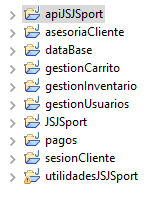
\includegraphics[width=0.3\linewidth]{conclusiones/imagenes/Proyecto}
	\caption{Estructura del proyecto en Eclipse}
\end{figure}

\subsection{Estructura del API}
\begin{figure}[th!]
	\centering
	\includegraphics[width=0.3\linewidth]{conclusiones/imagenes/EstructuraAPI}
	\caption{Estructura del API e interfaces}
\end{figure}
\newpage

\section{Prototipo pagina web}

\begin{figure}[th!]
	\centering
	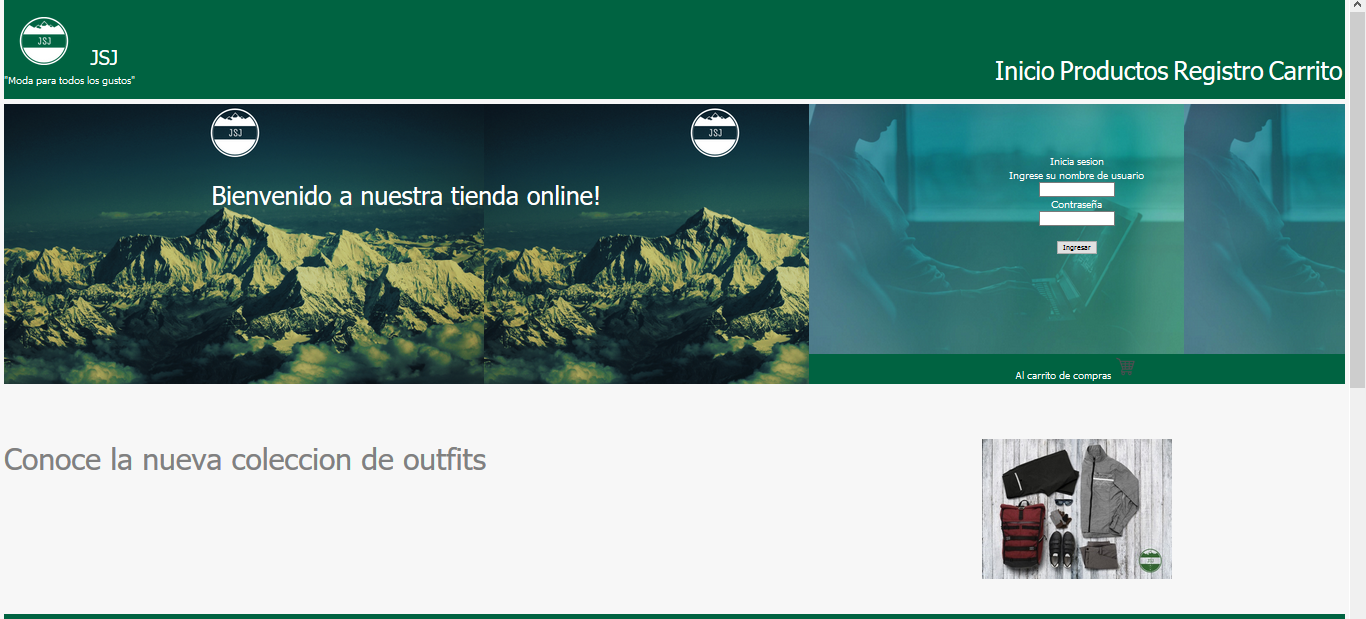
\includegraphics[width=1.0\linewidth]{conclusiones/imagenes/paginaWeb}
	\caption{Prototipo de la página web Inicio}
	
\end{figure}

\begin{figure}[th!]
	\centering
	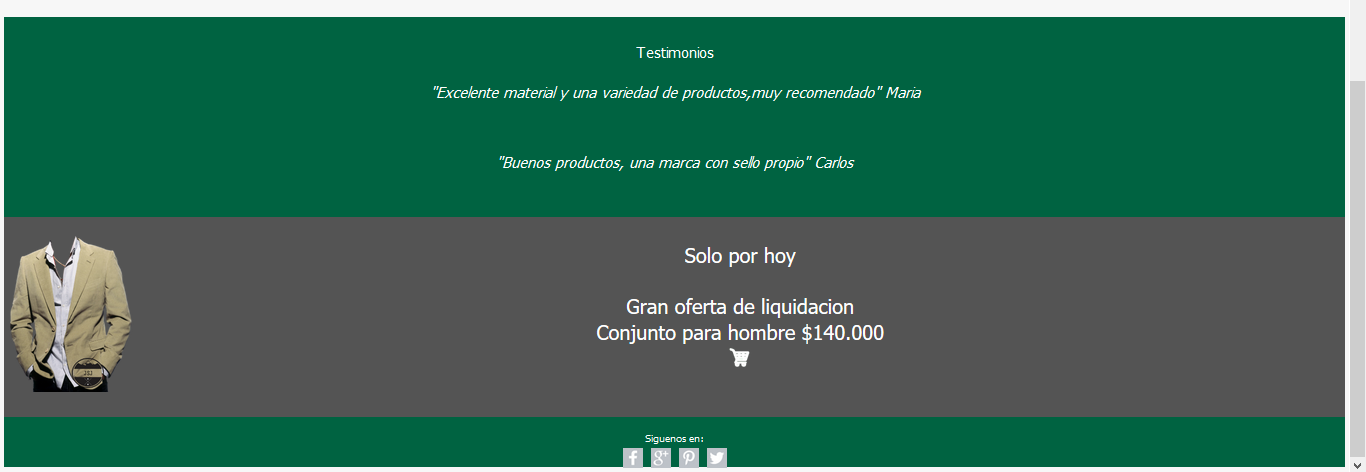
\includegraphics[width=1.0\linewidth]{conclusiones/imagenes/paginaWeb2}
	\caption{Prototipo de la página web Opiniones}
	
\end{figure}


\begin{figure}[th!]
	\centering
	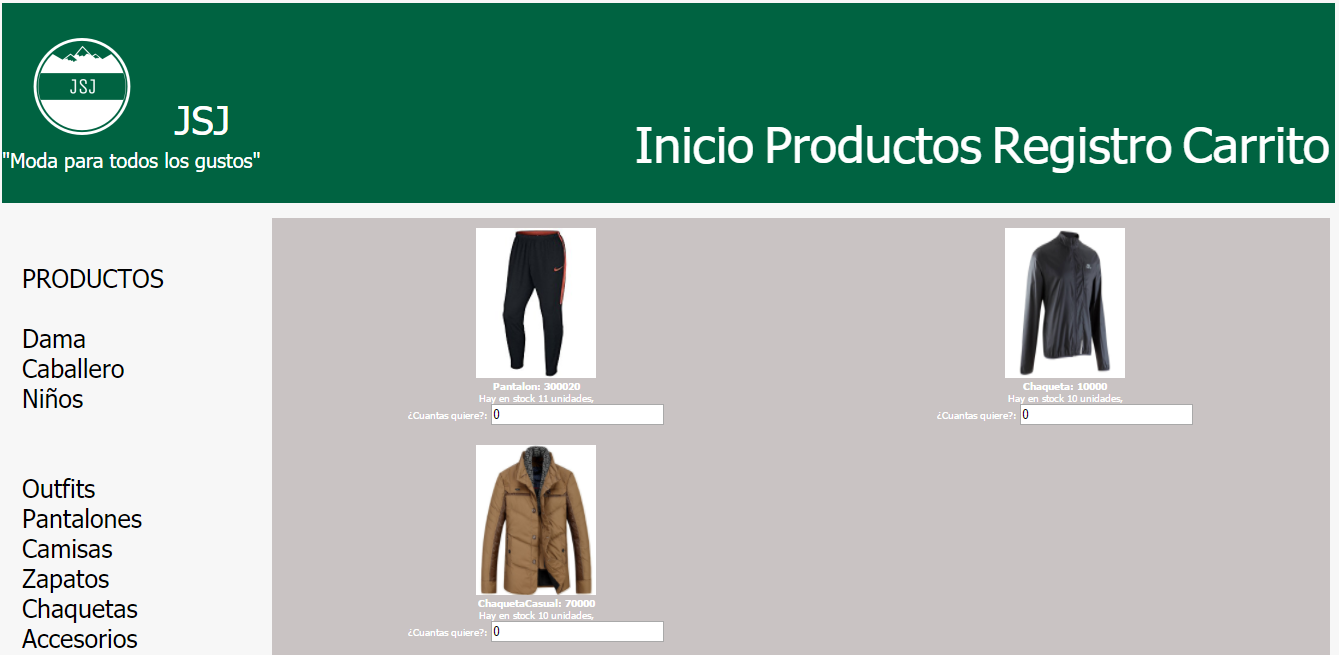
\includegraphics[width=0.7\linewidth]{conclusiones/imagenes/ProductosPaginaJSJ}
	\caption{JSJSports web Sección Productos}
\end{figure}

\begin{figure}[th!]
	\centering
	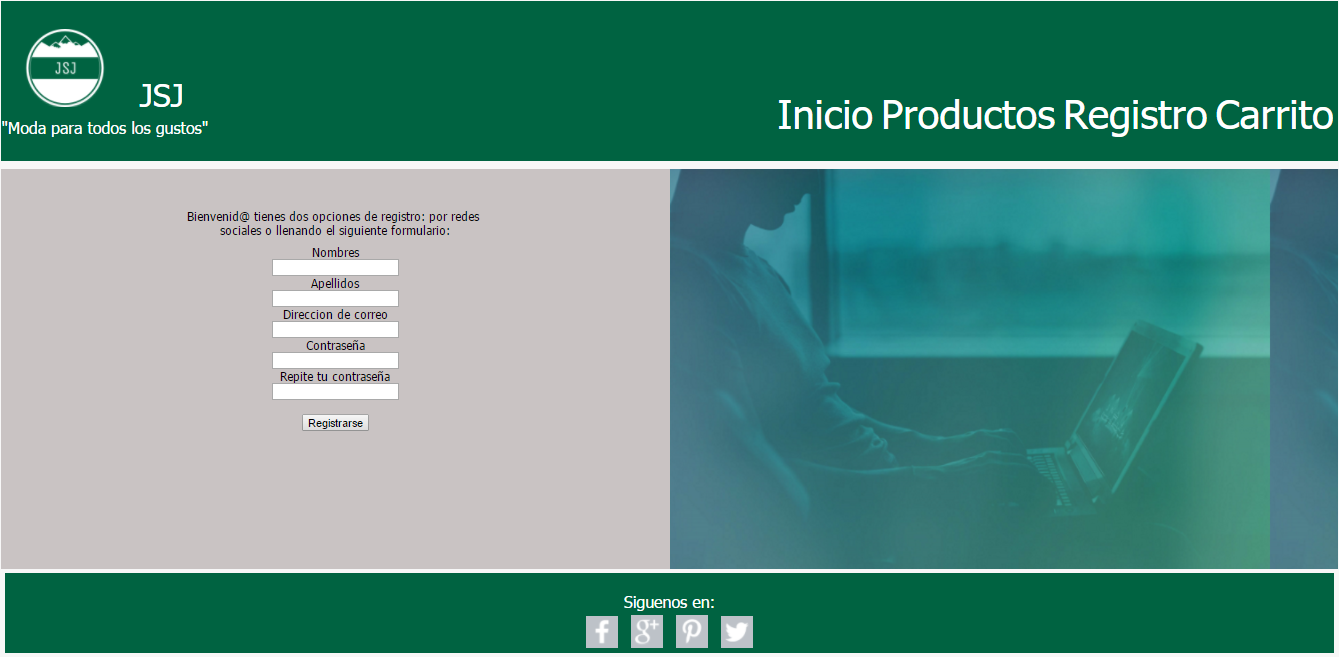
\includegraphics[width=0.7\linewidth]{conclusiones/imagenes/RegistroPaginaJSJ}
	\caption{JSJSports web Sección Registro de Usuario}
\end{figure}

\begin{figure}[th!]
	\centering
	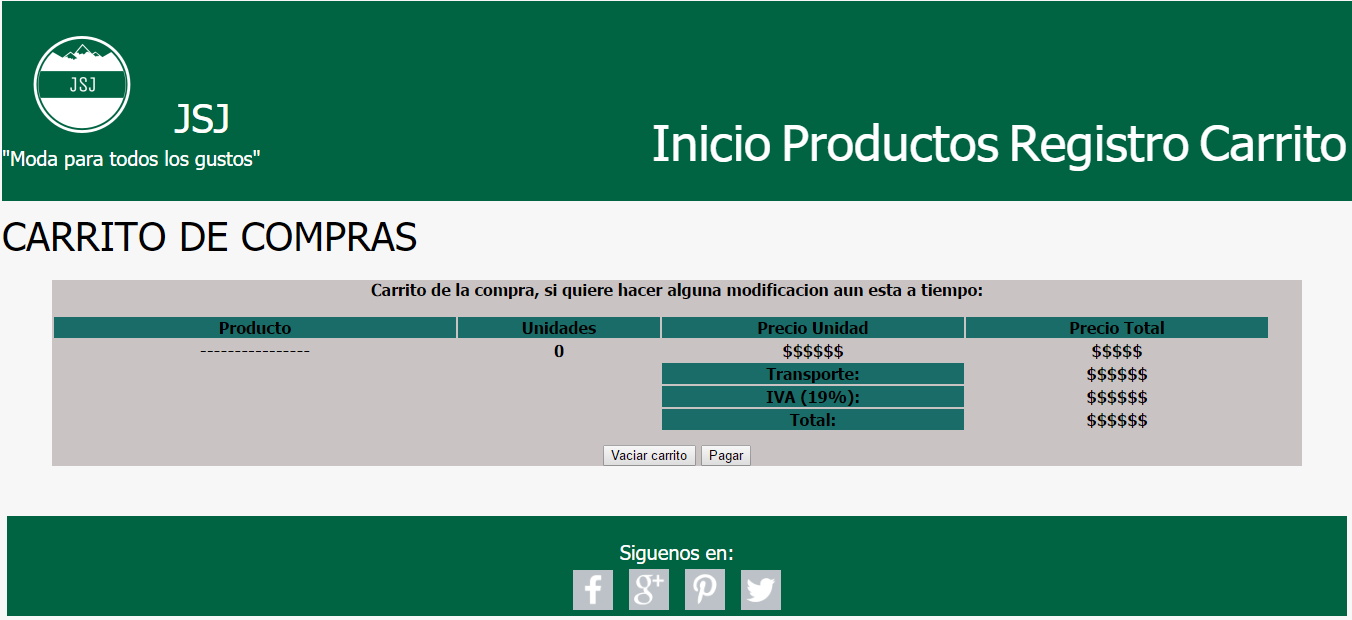
\includegraphics[width=0.7\linewidth]{conclusiones/imagenes/CarritoPaginaJSJ}
	\caption{JSJSports web Sección Carrito}
\end{figure}